\documentclass[../../tex_main/NEMO_manual]{subfiles}

\begin{document}

% ================================================================
% Chapter 7 � Ice thermodynamics
% ================================================================

\chapter{Ice thermodynamics}
\label{chap:THD}
\minitoc

\newpage
$\ $\newline    % force a new line


% ================================================================
% Thermodynamics % ================================================================

Mass, energy and salt are intertwined for sea ice. Referred to as thermodynamics, or more exactly halo-thermodynamics. Mushy-layer theory.

\section{Open water and new ice formation}

% There is everything in here, but there are too much details.
% Move things around into chapters and summarize.

As part of the sea ice computations, a heat budget of the uppermost oceanic level is estimated. This heat budget is used if negative to compute the production of new ice or, if positive, for bottom melting. 

%--------------------------------------------------------------------------------------------------------------------
%
% FIG x : Open water energy budget
%
\begin{figure}[ht]
\begin{center}
\vspace{0cm}
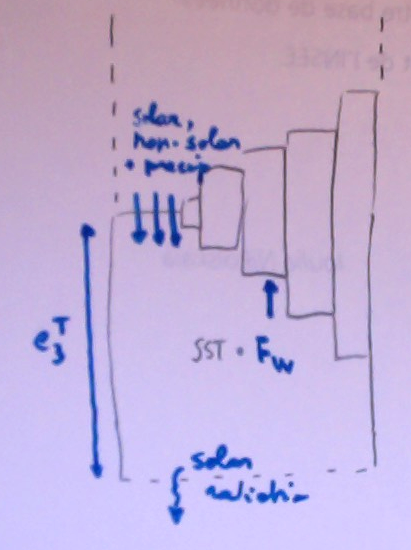
\includegraphics[height=10cm,angle=-00]{../Figures/Openwater_eb.png}
\caption{Scheme of the estimate of the heat budget of the first ocean level.}
\label{fig_yield}
\end{center}
\end{figure}
%
%--------------------------------------------------------------------------------------------------------------------

We estimate the heat budget of the first ocean level ($B^{opw}$) assuming four contributions, namely:
\begin{itemize}
\item The absorption of a fraction $f_1^{qsr}$ of solar radiation (given by radiative transfer component of the ocean model);
\item The non-solar heat flux absorbed at the surface;
\item The sensible heat content of precipitation
\item The sensible heat loss to the sea ice
\end{itemize}
The estimated heat budget thus reads:
\begin{linenomath}
\begin{align}
B^{opw} = Q^{sr} ( 1 - A ) f_1^{qsr} + Q^{ns} ( 1 - A ) + Q^{emp} - A F_w,
\end{align}
\end{linenomath}
Hence there is no consideration of the entrainment of heat at the base of the first ocean level, or of solar radiation transmitted below the ice. The ocean-to-ice turbulent sensible heat flux is formulated following \citep{McPhee92}
\begin{linenomath}
\begin{align}
F_w = \rho_0 c_w C_h u^* ( SST - T_b )
\end{align}
\end{linenomath}
where $\rho_0$ is the reference ocean density, $c_w$ is the seawater specific heat, $C_h = 7.5 \times 10^{-3}$ is a heat transfer coefficient, and $u^*=\sqrt{\tau_{iw}/\rho_0}$. There are two additional conditions, the oceanic heat flux cannot be negative. Second, $F_w$ cannot exceed the heat content of the first ocean level.

% Ice growth
If the $B^{opw}$ is such that the SST would decrease below the freezing point, the remainder of the heat is used to form new ice. The heat loss is converted into mass through [\ref{eq_phasechange}], giving by multiplication by density a volume of new ice $v_0$. The thickness $h_0$ of the new ice grown during a sea ice time step depends on unresolved small currents and waves and is prescribed. The fraction $a_0=v_0/h_0$ is computed accordingly. The salinity of this new ice $S_0$ is given by the S-h empirical relationship of \cite{Kovacs96}. The temperature assumed for this new ice is the local freezing point.

% Ice melt
If there is ice in the grid cell and that the $B^{opw}$ is positive, it is directly given attributed to the heat available for bottom melting. This argument follows from \cite{MaykutMcPhee95}, who found that most of solar heat absorbed in the surface waters is converted into melting. In practise, this means that the SST cannot go above freezing as long ice is present.

The heat loss used for ice formation, heat gain used to melt ice and the sensible heat given by the ocean to the ice, are all removed from the non-solar heat flux transmitted to the ocean.

Because ice dynamics are not able to maintain the small amount of open water that is observed, a maximum ice fraction ($amax, <1$) is prescribed.

\section{Diffusion of heat}

\section{Vertical growth and melt}

\section{Desalination}

\section{Remapping}

\section{Transport in thickness space}

\section{True lateral melting}

\end{document}

